\documentclass[tikz,border=10pt]{standalone}
\begin{document}
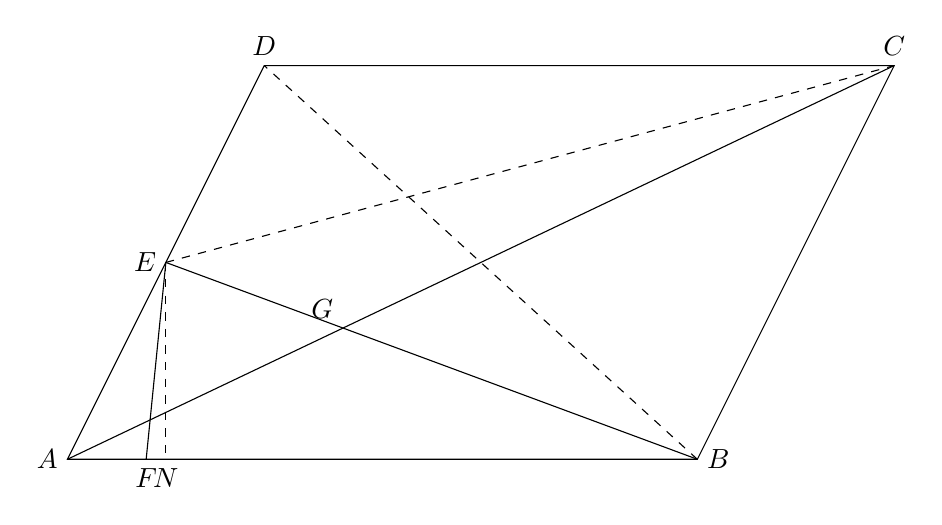
\begin{tikzpicture}
    \coordinate (A) at (0,0);
    \coordinate (B) at (8,0);
    \coordinate (C) at (10.5,5);
    \coordinate (D) at (2.5,5);
    \coordinate (E) at (1.25,2.5);
    \coordinate (F) at (1,0);
    \coordinate (N) at (1.25,0);
    \coordinate (G) at (3.5,1.67);

    \draw (A) -- (B) -- (C) -- (D) -- cycle;
    \draw (A) -- (C);
    \draw[dashed] (B) -- (D);
    \draw[dashed] (E) -- (C);
    \draw (E) -- (B);
    \draw (E) -- (F);
    \draw[dashed] (E) -- (N);

    \node[left] at (A) {$A$};
    \node[right] at (B) {$B$};
    \node[above] at (C) {$C$};
    \node[above] at (D) {$D$};
    \node[left] at (E) {$E$};
    \node[below] at (F) {$F$};
    \node[below] at (N) {$N$};
    \node[above left] at (G) {$G$};
\end{tikzpicture}
\end{document}
